\documentclass{beamer}
\usetheme{Madrid}
\usecolortheme{crane}


\usepackage[utf8]{inputenc}
\usepackage{adjustbox}
\usepackage{amsmath}
\usepackage{amssymb}
\usepackage{pbox}
\usepackage{subcaption}

\graphicspath{ {./images/}}

\DeclareMathOperator{\logit}{logit}


%Information to be included in the title page:
\title{Aiding Television Media Planning Through Bayesian Inference and Forecasting}
\author{Matthew Tiger}
\institute{Towson University}
\date{May 2018}


\begin{document}

\frame{\titlepage}

\frame{\tableofcontents}


\section{Introduction}

\begin{frame}
\frametitle{Background - TV Advertising Buying and Selling}

\begin{itemize}
\item
  The TV advertising landscape consists of TV sellers, who have airtime available
  for sale to be used to air advertisements, and TV buyers, who purchase airtime
  from TV sellers in order to air their desired advertisements.
\pause
\item TV sellers form \emph{media plans} based on the goals of TV buyers.
\pause
\item With each media plan, there is a certain number of guaranteed \emph{impressions} based off a declared buy-demographic.
\pause
\end{itemize}
\end{frame}

\begin{frame}{Background - TV Advertising Buying and Selling}
\begin{itemize}
\item To complicate the matter, the TV buyer may be interested in a sub-target audience and would want their advertising message to reach those additional people as well.
\pause
\item The TV seller must then provide forecasts for both targets and categorize the content according to what will efficiently target the sub-target audience. Inaccurate forecasts lead to either upset TV buyers or upset TV sellers.
\pause
\item The forecasts provided by the TV seller are based off audience measurement data. This data is based off of sampled data and could be noisy.
\end{itemize}
\end{frame}
\begin{frame}
\frametitle{Problem}

How can we forecast impressions of this sub-target given the forecasted impressions of the buy-demographic using noisy data?

\pause

Answer: \alert{Bayesian Inference!}
\end{frame}

\begin{frame}
\frametitle{Motivating Example: Baseball}
\begin{itemize}
  \item Baseball players are judged by their batting average (percentage of hits) but this metric is not informative when
  the player has few at-bats.
  \pause
  \item With more information about the league and past historical performances,
  we are able to come up with a better estimate through Bayesian inference.
  \pause
  \item
    Note that these estimates
  take into account the observed number of at-bats for each player
  which places larger evidence of skill, or lack thereof, on players with larger numbers of at-bats.
\end{itemize}
\end{frame}


\begin{frame}
\frametitle{Bayesian Inference}

\begin{itemize}
  \item Bayesian inference is the statistical practice that allows one to provide probability statements
    that express one's uncertainty on the occurrence of events and then learn about the parameters that determine those probabilities.

  \pause
\item A model for the data $y$ conditional on some unknown parameter $\theta$ is assigned
  as the \emph{likelihood} denoted by $p(y | \theta)$.
\pause
\item Based on prior knowledge some probability distribution is given to $p(\theta)$, i.e.\ the prior distribution for the parameter $\theta$.
\pause
\item Through the definition of conditional probability, we have that:

    \begin{align}\label{form:bayes}
      p(\theta | y) \propto p(y | \theta) p(\theta).
    \end{align}
\end{itemize}
\end{frame}


\section{Data}

\begin{frame}
\frametitle{Datasets}
\begin{itemize}
\item
  The data used to generate the forecasts come from two main sources TV suppliers and audience measurement companies.
\pause
\item TV suppliers provide the content that is set to air and the forecasted buy-demographic impressions
\pause
\item Audience measurement companies provide the measured historical impressions.
\pause
\item We will now discuss these datasets in more detail.
\end{itemize}
\end{frame}

\begin{frame}
\frametitle{Programming Schedule}
See below for sample records from the programming schedule provided by TV suppliers:
    \begin{table}[h!]
      \centering
      \begin{adjustbox}{width=1\textwidth,center=\textwidth}
        \large
        \begin{tabular}{lllllllll}
          network & selling title & selling title name & content & content name & start datetime & end datetime \\
          \hline
          BCST & 100 & Adult Cartoon 8PM & 10 & Adult Cartoon & 2017-04-02 20:00:00 & 2017-04-02 20:30:00 \\
          BCST & 101 & Adult Cartoon 8:30PM & 10 & Adult Cartoon & 2017-04-02 20:30:00 & 2017-04-02 21:00:00 \\
        \end{tabular}
      \end{adjustbox}
    \end{table}
\end{frame}

\begin{frame}
\frametitle{Forecasted Impressions}
Sample records from the forecasted impressions data provided by TV suppliers:
    \begin{table}[h!]
      \centering
        \begin{tabular}{llll}
          selling title & broadcast week & demographic & impressions per unit \\
          \hline
          100 & 2017-03-27 06:00:00 & F45-49 & 150000 \\
          100 & 2017-03-27 06:00:00 & P18-49 & 1500000 \\
          101 & 2017-03-27 06:00:00 & F45-49 & 120000 \\
          101 & 2017-03-27 06:00:00 & P18-49 & 1000000 \\
        \end{tabular}
    \end{table}

\end{frame}

\begin{frame}
\frametitle{Audience Measurement - Programs}
Sample records from Audience Measurement Programs Data:
  \begin{table}[h!]
    \centering
    \begin{adjustbox}{width=1\textwidth,center=\textwidth}
      \large
      \begin{tabular}{lllllllllll}
        airing & network & program & telecast & program name & start datetime & end datetime & genre & is first run & is live\\
        \hline
        35 & BCST & 1000 & 301 & Adult Cartoon & 2017-04-02 20:02:00 & 2017-04-02 20:30:00 & Animation & 1 & 0 \\
        36 & BCST & 1000 & 302 & Adult Cartoon & 2017-04-02 20:30:00 & 2017-04-02 21:00:00 & Animation & 1 & 0
      \end{tabular}
    \end{adjustbox}
  \end{table}


\end{frame}

\begin{frame}
\frametitle{Audience Measurement - Viewing}
Sample records from Audience Measurement Viewing Data:
  \begin{table}[h!]
    \centering
    \begin{adjustbox}{width=0.8\textwidth,center=\textwidth}
      \large
    \begin{tabular}{lllllllll}
      program & telecast & respondent & minute & comm secs & weight & age & gender & total comm secs\\
      \hline
      1000 & 301 & 2 & 3 & 60 & 2050 & 48 & F & 120\\
      1000 & 301 & 2 & 4 & 45 & 2050 & 48 & F & 120\\
      1000 & 301 & 2 & 15 & 60 & 2050 & 48 & F & 120\\
      1000 & 301 & 2 & 16 & 30 & 2050 & 48 & F & 120\\
      1000 & 302 & 2 & 22 & 15 & 2050 & 48 & F & 100\\
      1000 & 302 & 2 & 23 & 60 & 2050 & 48 & F & 100
    \end{tabular}
    \end{adjustbox}
  \end{table}
\end{frame}

\begin{frame}
  \frametitle{Audience Measurement - Measurements}
  \begin{itemize}
    \item The impressions associated to a telecast is given by the Average Commercial Minute (ACM).
      \pause
      \item This is the weighted sum of the commercial viewing of a target over the total number of commercial seconds.
        \pause
      \item Define $m_{i}^A$, the ACM of target A for airing $i$ as follows:
  \begin{align}\label{acm_def}
    m_{i}^A = \left\lceil\frac{\sum_{k=1}^n w_k \sum_{j=1}^{t_i} s_{ij} p_{ijk} \textbf{1}_A(p_{k})}{\sum_{j=1}^{t_i} s_{ij}}\right\rceil.
  \end{align}
\end{itemize}
\end{frame}


\begin{frame}
\frametitle{Training Data}

\begin{itemize}
  \item We limit the data from the above data sets to three networks labeled BCST, ETMT, and SPTS during broadcast years 2016 - 2017.
  \item We consider the in-target audience, target $A$, to be Females aged 45 - 49 and the buy-demographic audience, target $B$,
    to be Persons aged 18-49.
  \item We combine the information from the above data sets to form the training data:
  \begin{table}[h!]
    \centering
    \begin{adjustbox}{width=0.9\textwidth}
      \large
      \begin{tabular}{llllllllll}
        network & selling title & content & start datetime & end datetime & program & telecast & ACM A & ACM B\\
        \hline
        BCST & 100 & 10 & 2017-04-02 20:00:00 & 2017-04-02 20:30:00 & 1000 & 301 & 110560 & 1203560\\
        BCST & 101 & 10 & 2017-04-02 20:30:00 & 2017-04-02 21:00:00 & 1000 & 302 & 210560 & 1501000\\
      \end{tabular}
    \end{adjustbox}
  \end{table}
\end{itemize}
\end{frame}

\begin{frame}
\frametitle{Audience Size Comparison}
\begin{figure}[!h]
  \centering
  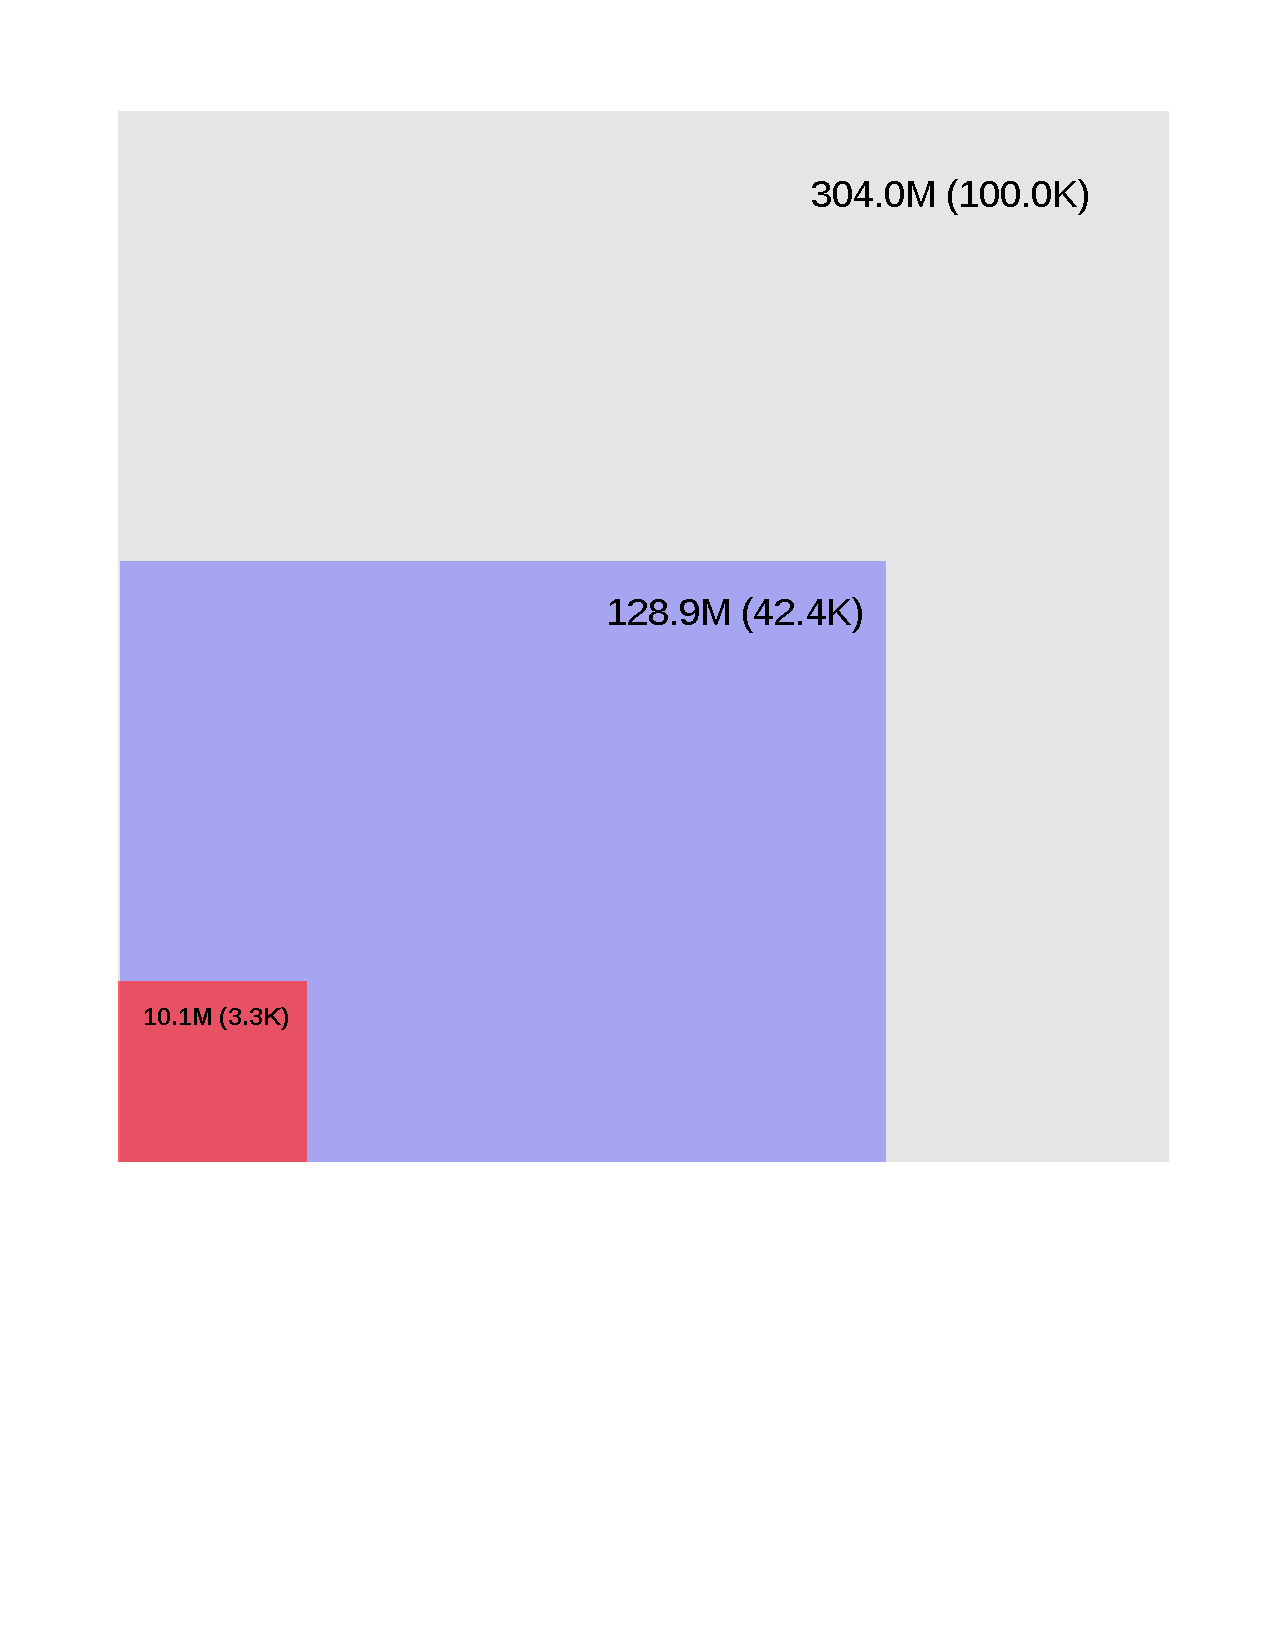
\includegraphics[scale=0.35]{panel}
\end{figure}
\end{frame}


\section{Model}

\begin{frame}
\frametitle{Units of Observation}
\begin{itemize}
  \item The units of observation for this model are individual content airings in the media schedule.
    \pause
  \item The outcome variable that is measured for each unit $i$ is $m_i^A$, the ACM of target $A$, which we
    denote as $y_i$ for notational convenience.
    \pause
  \item Similarly, we denote $m_i^B$, the ACM of target $B$ for unit $i$ by $n_i$.
\end{itemize}

\end{frame}

\begin{frame}
\frametitle{Covariates}
\begin{itemize}
  \item \emph{Time-based} covariates and \textbf{Program-based} covariates
  \pause
  \item Derived from Media Schedule
    \begin{itemize}
      \item \emph{Broadcast Month}
      \item \emph{Day of Week}
      \item \emph{Stratified Hour}
      \item \textbf{Content}
      \item \textbf{Lead-in Content}
    \end{itemize}
  \pause
  \item Derived from Audience Measurement Data
    \begin{itemize}
      \item \textbf{Genre}
      \item \textbf{Live-program}
      \item \textbf{First-run}
    \end{itemize}

\end{itemize}

\end{frame}

\begin{frame}
\frametitle{Assumptions}
\begin{itemize}
  \item We assume that the response variables $y_i$ are \emph{exchangeable} given the parameters of the model
  and the covariates of the unit of observation.

  \pause
  \item A sequence of random variable is exchangeable if the ``joint probability density $p(y_1, \dots, y_k)$ is invariant to permutations of the indexes.''
  \pause
  \item This allows us to model the data as independently and identically distributed given the covariates and unknown parameters.

\note[item]{This means the order in which the data occurs does not determine the joint probability density and therefore is unimportant.}
\end{itemize}
\end{frame}

\begin{frame}
\frametitle{Model Description}
Define model $\mathcal{M}$ to be
\begin{align*}
  y_i | X_i, n_i, \pi_i, \omega_i, \kappa_i &\sim \text{Bin}(n_i, \pi_i) \\
  \pi_i | \omega_i, \kappa_i &\sim \text{Beta}\left(\omega_i \kappa_i + 1, (1 - \omega_i) \kappa_i + 1\right) \\
  \omega_i &= \logit^{-1}\left(\beta_0 + \sum_{j=1}^{m-1}  \beta_j X_{ij}\right), \quad \beta_j \sim t_4(0, \sigma_j^2) \\&\quad \text{for $0 \leq j \leq m$}\\
  \kappa_i | X_{im} &\sim \text{Exp}(\lambda_p X_{im}), \quad \text{for $p = 0, 1$},
\end{align*}
where $\logit^{-1}(\alpha) = \frac{\exp{\alpha}}{1 + \exp{\alpha}}$.

\end{frame}

\begin{frame}
\frametitle{Model Description}
\begin{figure}[!h]
  \centering
  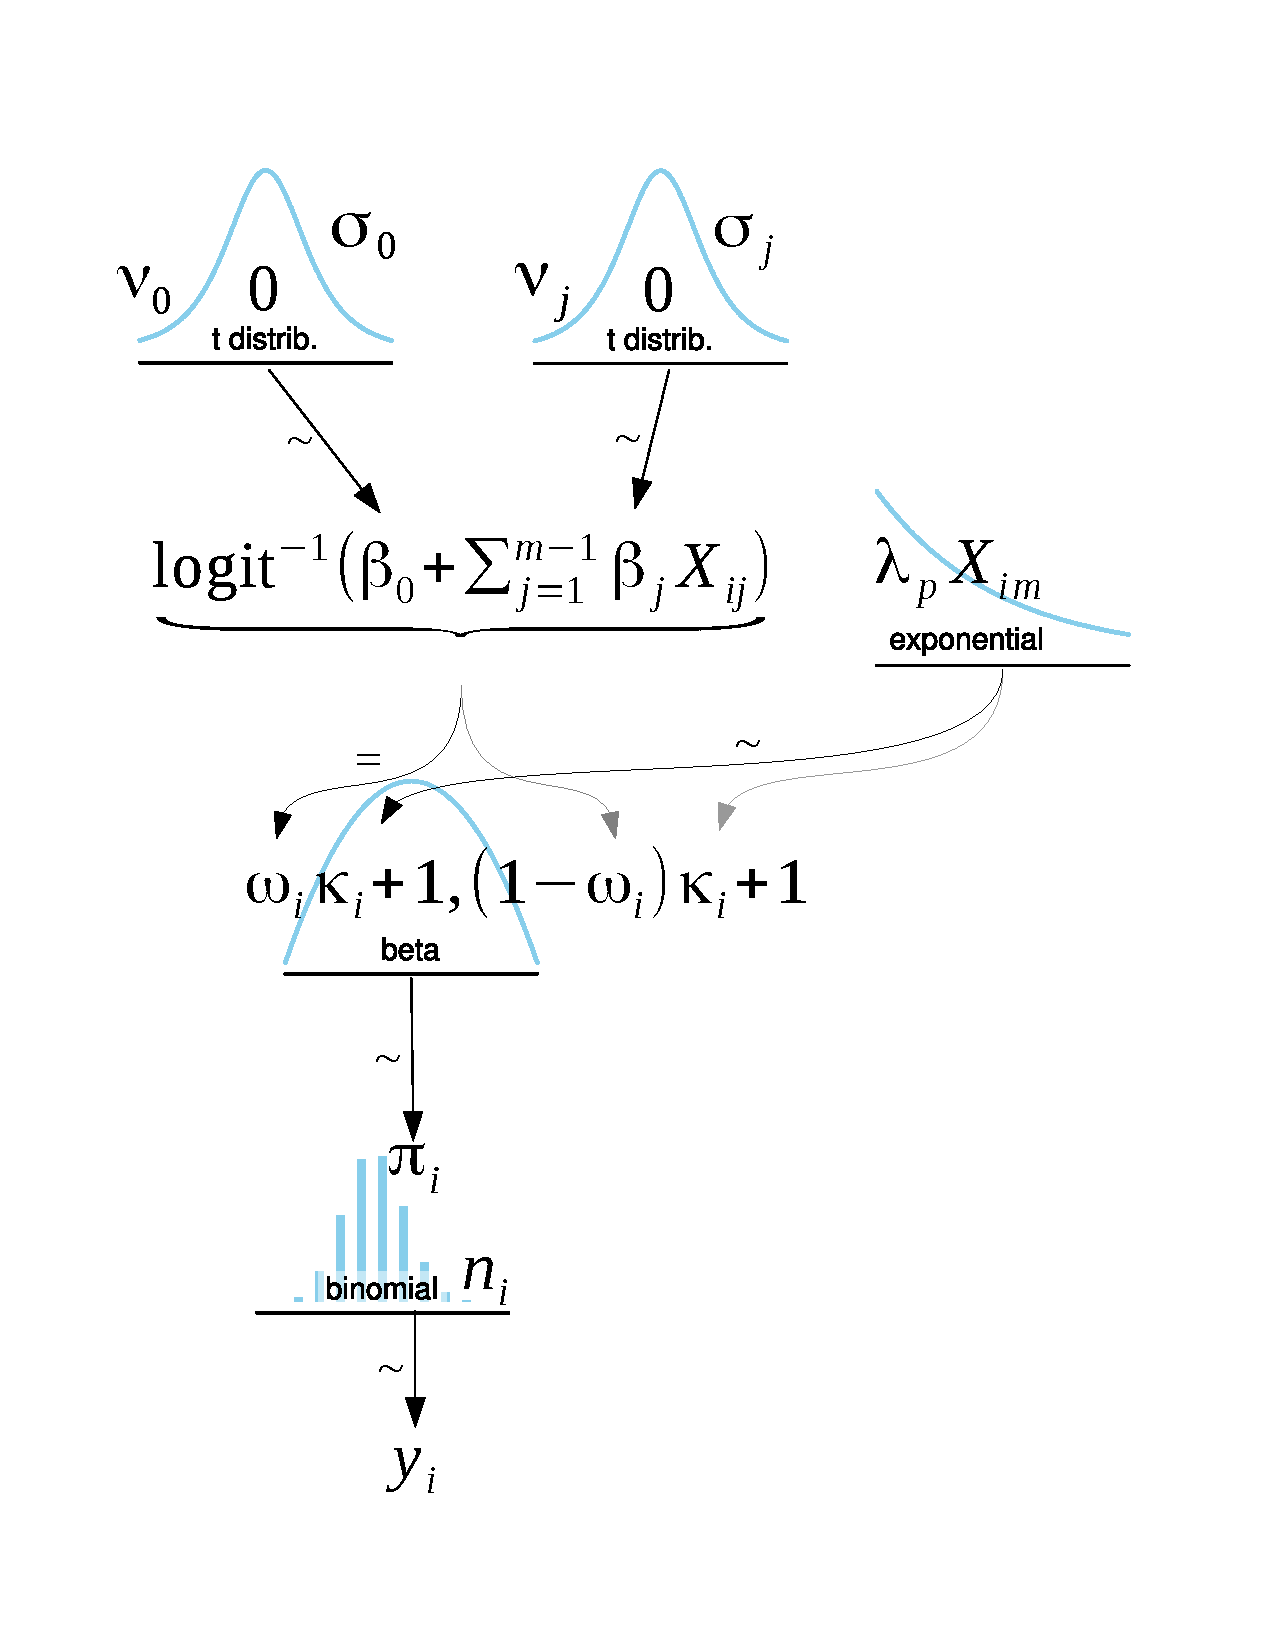
\includegraphics[scale=0.3]{kruschke_diagram}
\end{figure}
\end{frame}

\begin{frame}
\frametitle{Prior Distribution Choice}
\begin{itemize}
\item Prior distributions for coefficients $\beta_j$ and concentration parameter $\kappa_i$ are chosen to be \emph{weakly informatative}.
\pause
\item For the coefficients, this means that $\mu_j=0, \nu_j = 4$ for all $j$ and that $\sigma_j = 2.5$ if $1 \leq j \leq m$ otherwise $\sigma_0 = 5$.
\pause
\item For the concentration parameter, this means that $\lambda_p = 10^{-4}$.
\pause
  \begin{figure}[h!]
    \begin{center}
      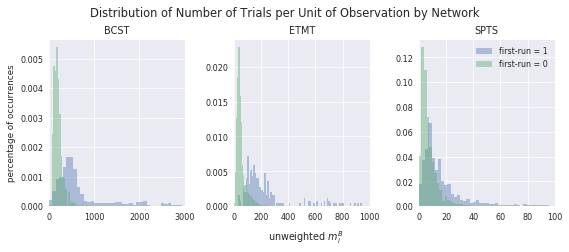
\includegraphics[scale=0.4]{kappa_explanation}
    \end{center}
  \end{figure}

\note[item]{Weakly informative here means that the priors are ``intentionally weaker than whatever prior
knowledge is available'' and act as constraints on the possible parameters that are to be sampled.}
\note[item]{This means $\beta_1, \dots, \beta_m$ are between -5 and 5 which on the logit scale are roughly 0.01 and 0.99
which is a larger effect than is to be expected by a single coefficient. We use weaker prior on intercept since more information
is available about intercept through data. Mean 0 is chosen because apriori we don't know if coefficient will be positive or negative.
}
\note[item]{Panel size is $10^5$ so $\lambda_p = 10^{-4}$ allows for parameter to be equal to total number of panelists.}
\end{itemize}
\end{frame}


\begin{frame}
\frametitle{Computation}
\begin{itemize}
\item Inference was computed using pymc3, a probabilistic programming language and library for Python.
\pause
\item The library is powered by the No U-Turn Sampler (NUTS) which is a variant of Hamiltonian Monte Carlo (HMC).
\pause
\item Parameters used for sampling:
  \begin{itemize}
    \item \texttt{target\_accept}: 0.95
    \item tuned samples: 3000
    \item drawn samples: 500
    \item number of chains: 4
  \end{itemize}
\end{itemize}
\end{frame}

\begin{frame}
\frametitle{Convergence}

\begin{itemize}
\item Approximate convergence to posterior distribution is measured through the \emph{Gelman-Rubin} statistic, denoted by $\hat{R}$.
\pause
\item Another convergence check is the number of effective samples produced by the simulation, denoted by $\hat{n_{\text{eff}}}$.
\pause
\item If $\hat{R}$ is close to 1 then we may assume we have approximate convergence. Further it is recommended that $\hat{n_{\text{eff}}} \geq 10 M$ where $M$ is the number of sampled Markov chains for all model parameters.
\pause
\item For each network model, we have that $0.99 \leq \hat{R} \leq 1.01$ and $\hat{n_{\text{eff}}} > 400$
    for all model parameters.

\note[item]{This is a measure of the between-sequence and within-sequence variance
  across the Markov chains and is used to determine if stationarity and mixing has been achieved.}
\note[item]{Number of effective samples is measured through the autocorrelation of the Markov Chain at lag $t$. More autocorrelation means less effective samples.}
\end{itemize}
\end{frame}


\section{Model Fit}

\begin{frame}
\frametitle{Posterior Predictive Checks}
\begin{itemize}
  \item ``If the model fits, then replicated data under the model should look similar
  to observed data.''
  \pause
  \item Generating data using the posterior density and checking some aspect of the generated data set is called a
    \emph{posterior predictive check}.
\end{itemize}
\pause
Let $y$ be the observed data and $\theta$ be the vector of model parameters. Define $y^{\text{rep}}$ to be the replicated data
that could have been generated given $\theta$, i.e.\

\begin{align}\label{form:yrep}
    p(y^{\text{rep}} | y) = \int p(y^{\text{rep}}|\theta)p(\theta | y) d\theta.
\end{align}
\note[item]{Note the replicated data is dependent on the data. This formula marginalizes out the vector of parameters.}
\end{frame}

\begin{frame}
\frametitle{Replicated versus Actual Data}
\begin{figure}
  \begin{subfigure}{.75\textwidth}
    \centering
    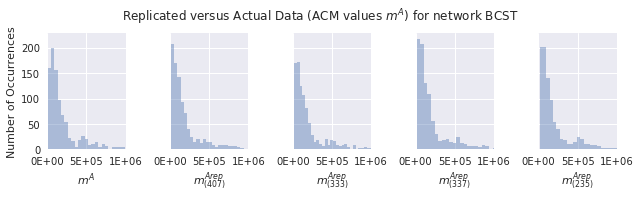
\includegraphics[scale=0.35]{BCST_m_rep}
  \end{subfigure}
  \begin{subfigure}{.75\textwidth}
    \centering
    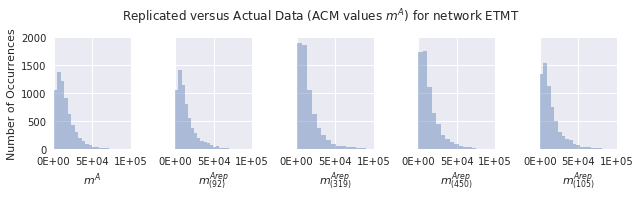
\includegraphics[scale=0.35]{ETMT_m_rep}
  \end{subfigure}
  \begin{subfigure}{.75\textwidth}
    \centering
    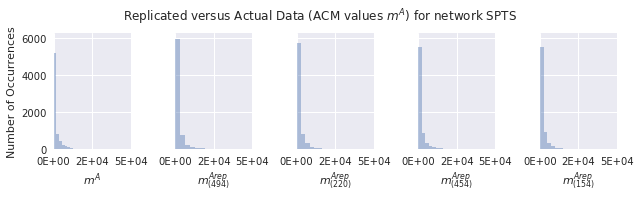
\includegraphics[scale=0.35]{SPTS_m_rep}
  \end{subfigure}
\end{figure}
\end{frame}

\begin{frame}
\frametitle{Replicated versus Actual Data}
    \begin{figure}[!h]
      \begin{subfigure}[b]{.75\textwidth}
        \centering
        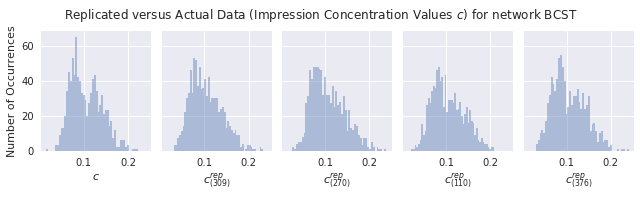
\includegraphics[scale=0.35]{BCST_c_rep}
      \end{subfigure}
      \begin{subfigure}[b]{.75\textwidth}
        \centering
        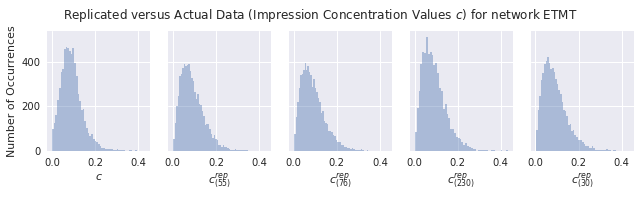
\includegraphics[scale=0.35]{ETMT_c_rep}
      \end{subfigure}
      \begin{subfigure}[b]{.75\textwidth}
        \centering
        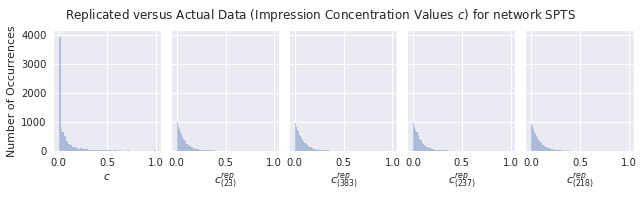
\includegraphics[scale=0.35]{SPTS_c_rep}
      \end{subfigure}
    \end{figure}
\end{frame}

\begin{frame}
\frametitle{Test Statistics}
\begin{itemize}
\item We can quantify model discrepancies by defining a test quantity $T(y, \theta)$
    and then measuring the discrepancy between the observed data and the replicated data.
\pause
\item Formally, we can compute a posterior predictive $p$-value defined as
\begin{align*}
  p_B = \text{Pr}\left( T(y^{\text{rep}}, \theta) \geq T(y, \theta)  | y \right).
\end{align*}
\pause
\item Since we use simulated values of the posterior density, we have that the estimated
$p$-value for $S$ simulations is given by:
\begin{align}
  \hat{p_B} = \frac{1}{S}\sum_{i=1}^S [T(y_{(i)}^{\text{rep}}, \theta_{(i)}) \geq T(y, \theta_{(i)})].
\end{align}

\end{itemize}
\end{frame}

\begin{frame}
\frametitle{Test Statistics - Definition}
We define the following test quantities to use in evaluating the fit of model $\mathcal{M}$:
\begin{itemize}
\item $T_1(y, \theta):= \min(y)$,
\pause
\item $T_2(y, \theta):= \overline{y} = \frac{1}{N}\sum_{i=1}^N y_i$,
\pause
\item $T_3(y, \theta):= \max(y)$,
\pause
\item $T_4(y, \theta):= \text{std}(y) = \sqrt {\frac {\sum _{i=1}^{N}(y_{i}- \overline {y})^{2}}{N-1}}$.
\end{itemize}
\end{frame}

\begin{frame}
  \frametitle{Test Statistics - Evaluation - BCST network}
  \centering
      \begin{tabular}{lrcccccccc}
        Test quantity & $T(y, \theta)$ & \pbox{2cm}{95\% int. for $T(y^{\text{rep}}, \theta)$} & $p_B$ \\ \\
        \hline \\
        $T_1(y, \theta)$ (min) & 3701 & [6245, 14270] & 0.99 \\
        $T_2(y, \theta)$ (mean) & 227457.84 & [2266852.49, 236367.09] & 0.95 \\
        $T_3(y, \theta)$ (max) & 4311038 & [3443885, 4989241] & 0.34 \\
        $T_4(y, \theta)$ (std) & 334052.86 & [325128.37, 364859.10] & 0.90
      \end{tabular}
\end{frame}

\begin{frame}
  \frametitle{Test Statistics - Evaluation - ETMT network}
  \centering
      \begin{tabular}{lrcc}
        Test quantity & $T(y, \theta)$ & \pbox{2cm}{95\% int. for $T(y^{\text{rep}}, \theta)$} & $p_B$ \\ \\
        \hline \\
        $T_1(y, \theta)$ (min) & 0 & [9, 182] & 1.0 \\
        $T_2(y, \theta)$ (mean) & 16357.80 & [16705.39, 17489.11] & 1.0 \\
        $T_3(y, \theta)$ (max) & 452762 & [307901, 760822] & 0.78  \\
        $T_4(y, \theta)$ (std) & 17686.89 & [20021.24, 23205.09] & 1.0
      \end{tabular}
\end{frame}

\begin{frame}
  \frametitle{Test Statistics - Evaluation - SPTS network}
  \centering
  \begin{tabular}{lrcc}
    Test quantity & $T(y, \theta)$ & \pbox{2cm}{95\% int. for $T(y^{\text{rep}}, \theta)$} & $p_B$\\ \\
    \hline \\
    $T_1(y, \theta)$ (min) & 0 & [0, 0] & 1.0 \\
    $T_2(y, \theta)$ (mean) & 3972.45 & [3714.91, 4559.66] & 0.73 \\
    $T_3(y, \theta)$ (max) & 526816 & [607186, 2239365] & 0.99 \\
    $T_4(y, \theta)$ (std) & 22300.18 & [20012.59, 39808.44] & 0.88
  \end{tabular}

\end{frame}

\begin{frame}
\frametitle{Residual Analysis}
\begin{itemize}
    \item For a model with unknown parameters $\theta$ and predictors $x_i$, the \emph{predicted}
    value is $\text{E}(y_i | x_i, \theta)$ and the \emph{residual} is $r_i = y_i - \text{E}(y_i | x_i, \theta)$.
    \pause
    \item The \emph{standardized residual} is given by $r_i / \text{std}(y)$.
    \pause
    \item Using the simulated posterior density, we can compute $\text{E}(y_i | x_i, \theta)$
    to be the mean of the replicated hold-out data itself.
\end{itemize}
\end{frame}

\begin{frame}
\frametitle{Residual Analysis - Actual versus Replicated}
    \begin{figure}[!h]
      \begin{subfigure}[b]{.75\textwidth}
        \centering
        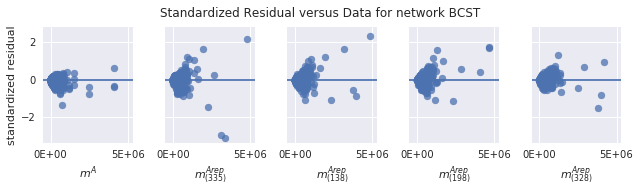
\includegraphics[scale=0.33]{BCST_res}
      \end{subfigure}
      \begin{subfigure}[b]{.75\textwidth}
        \centering
        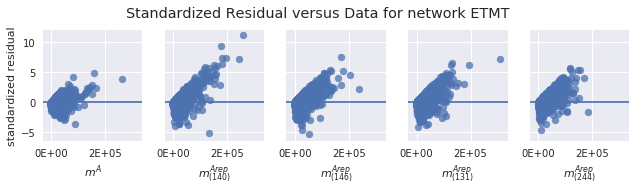
\includegraphics[scale=0.33]{ETMT_res}
      \end{subfigure}
      \begin{subfigure}[b]{.75\textwidth}
        \centering
        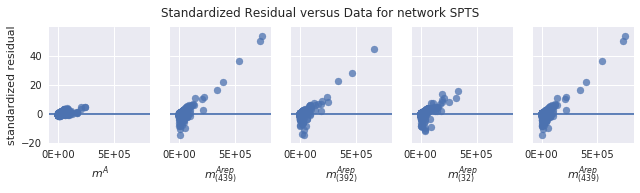
\includegraphics[scale=0.33]{SPTS_res}
      \end{subfigure}
    \end{figure}
\end{frame}


\begin{frame}
\frametitle{Residual Analysis - Test Statistic Evaluation}
    We can measure the residual mis-fit through the following test statistic:
    \begin{align*}
      T(y, \theta, x) = \frac{\overline{r}}{\text{std}(y)}.
    \end{align*}
    \pause
    \begin{figure}[!h]
      \begin{subfigure}[b]{.32\textwidth}
        \centering
        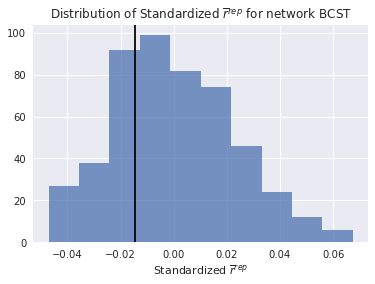
\includegraphics[scale=0.3]{BCST_res_test}
      \end{subfigure}
      \begin{subfigure}[b]{.32\textwidth}
        \centering
        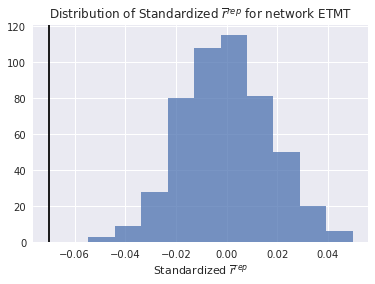
\includegraphics[scale=0.3]{ETMT_res_test}
      \end{subfigure}
      \begin{subfigure}[b]{.32\textwidth}
        \centering
        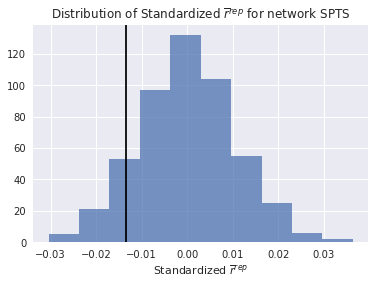
\includegraphics[scale=0.3]{SPTS_res_test}
      \end{subfigure}
    \end{figure}
\end{frame}
\section{Results}

\begin{frame}
\frametitle{Industry Standard Model}

\begin{itemize}
\item The industry standard model used today to forecast impressions is based on the average of observed data.
\pause
\item Define model $\mathcal{M}_0$ to be as follows:
  \begin{enumerate}
    \item Using the content and stratified hour, take the average impression concentration $c_i$ of the train set.
    \item Using the stratified hour, take the average impression concentration $c'_i$ of the train set.
    \item The forecasted $m_i^A$ for airing $i$ is then $c_i m_i^B$ if it exists, otherwise it is $c_i' m_i^B$.
  \end{enumerate}
\pause
\item We wish to compare the performance of model $\mathcal{M}$ to model $\mathcal{M}_0$ and determine
  if the proposed model outperforms the industry standard model.
\end{itemize}
\end{frame}

\begin{frame}
\frametitle{Analysis - Error Metrics}
\begin{itemize}
  \item The main error metric we will use to evaluate model performance is the Mean Absolute Error. It is defined as
    \begin{align*}
      MAE = \frac{1}{N}\sum_{i=1}^N|y_i^{\text{act}} - y_i^{\text{pred}}|
    \end{align*}
  \pause
  \item Additionally, we can use an analogous metric to evaluate the probabilistic forecasts called
    the Continuous Ranked Probability Score (CRPS).
\pause
\item Let $F$ be the cumulative distribution function of a random variable $X$
    and $x$ be the observed value. Then we have that:
    \begin{align}\label{form:crps}
      \text{CRPS}(F, x) = \int_{-\infty}^{\infty}\left(F(y) - H(y - x)\right)^2dy
    \end{align}
    Note that this is a generalization of the Mean Absolute Error.
\end{itemize}
\end{frame}

\begin{frame}
\frametitle{Analysis - Calibration}
\begin{itemize}
  \item We are also interested in the \emph{calibaration} of the forecasted probability distributions.
    \pause
  \item We can assess the calibration of the probabilistic forecasts by calculating
    Credible Regions (CRs) for each unit of observation and determining the proportion of units
    that fall within the CRs compared to the number of units.
  \pause
    \item The forecasts are perfectly calibrated if for a CR of $(1 - \alpha)\%$, the proportion of units
    within the CR is $(1-\alpha)\%$.
\end{itemize}
\end{frame}

\begin{frame}
\frametitle{Analysis - Units of Observation}
\begin{itemize}
  \item The table below shows the evaluation of error metrics between the models:
    \begin{table}[h!]
      \centering
      \begin{tabular}{lrrrr}
        network & $\overline{m_i^A}$ & $\mathcal{M}_0$ MAE & $\mathcal{M}$ CRPS & $\mathcal{M}$ MAE \\
        \hline
        BCST & 171450.06 & 23307.81 & 15247.91 & 21408.24 \\
        ETMT & 13034.77 & 5123.70 & 3683.04 & 5226.42 \\
        SPTS & 3164.84 & 1844.51 & 1426.60 & 1942.76
      \end{tabular}
    \end{table}
  \item The point-forecasts of Model $\mathcal{M}$ perform on-par with, or slightly worse than $\mathcal{M}_0$.
  \pause
  \item However, the probabilistic forecasts of model $\mathcal{M}$ greatly outperform model $\mathcal{M}_0$.
\end{itemize}

\end{frame}

\begin{frame}
\frametitle{Analysis - Units of Observation}
The table below shows the calibration of the probabilistic forecasts at the level
of the units of observation.
\begin{table}[h!]
  \centering
  \begin{tabular}{lrrr}
    & \multicolumn{3}{c}{Credible Region $(1 - \alpha)\%$} \\
    network & $\alpha = 0.5$ & $\alpha = 0.05$ & $\alpha = 0.01$ \\
    \hline
    BCST & 0.465 & 0.922 & 0.966 \\
    ETMT & 0.48 & 0.91 & 0.95  \\
    SPTS & 0.416 & 0.765 & 0.799 \\
  \end{tabular}
\end{table}
\end{frame}

\begin{frame}
\frametitle{Analysis - Units of Observation - SPTS}

\begin{itemize}
  \item Closer analysis reveals that the right-censored data is causing the miscalibration
    on the SPTS network.
    \pause
  \item The figure below shows the distribution of lower-limits of 95\% CRs in which
    the outcome was outside the above specified CRs:
    \begin{figure}[!h]
      \centering
      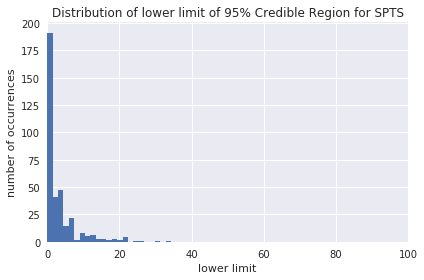
\includegraphics[scale=0.4]{SPTS_CR_analysis}
    \end{figure}
  \item Removing the right-censored data and recalculating the $95\%$ CRs shows that
    91.8\% of units are within the forecasted CR, consistent with other networks.
\end{itemize}

\end{frame}

\begin{frame}
\frametitle{Quantiled Media Plans}

\begin{itemize}
  \item We are interested in understanding the performance of aggregations of units of observation
    since these aggregations form the media plans.
    \pause
  \item To do this, we quantile the units in the hold-out set into 20 bins ordered by the point forecasts
    of the impression concentration as a proxy for creating media plans. We then compute the total forecasted
    impressions of the media plan using each model.
   \pause
  \item For model $\mathcal{M}_0$, the total forecasted impressions are the sum of the individual point forecasts.
    \pause
  \item For model $\mathcal{M}$, under the model assumptions, the units are i.i.d.\ given the covariates and parameters.
    We can create the distribution of aggregated impressions through simple sums of the distributions of outcomes at the level of the units of observation.
\end{itemize}
\end{frame}

\begin{frame}
\frametitle{Quantiled Media Plans}
    \begin{figure}[!h]
      \centering
      \begin{subfigure}[b]{.75\textwidth}
        \centering
        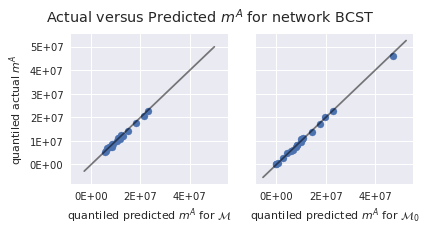
\includegraphics[scale=0.3]{BCST_quantiled}
      \end{subfigure}
      \begin{subfigure}[b]{.75\textwidth}
        \centering
        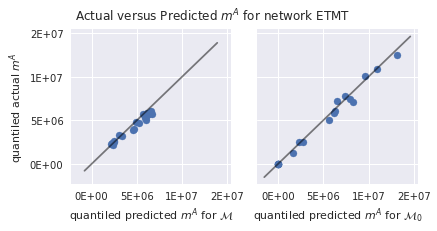
\includegraphics[scale=0.3]{ETMT_quantiled}
      \end{subfigure}
      \begin{subfigure}[b]{.75\textwidth}
        \centering
        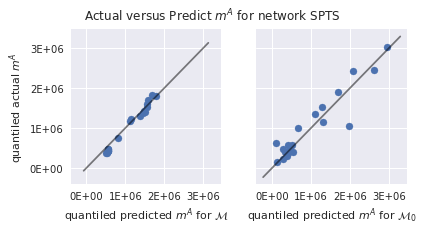
\includegraphics[scale=0.3]{SPTS_quantiled}
      \end{subfigure}
    \end{figure}
\end{frame}


\begin{frame}
  \frametitle{Quantiled Media Plans - Error Metrics}
  \begin{itemize}
    \item
      The table below shows the error metrics between the two models for the quantiled media plans.
    \begin{table}[h!]
      \centering
        \begin{tabular}{lrrrr}
          network  & $\mathcal{M}_0$ MAE & $\mathcal{M}$ CRPS & $\mathcal{M}$ MAE \\
          \hline
          BCST & 324034.14 & 277437.29 & 417797.60 \\
          ETMT & 297512.52 & 311316.38 & 399648.10 \\
          SPTS & 205096.15 & 75962.55 & 90668.35
        \end{tabular}
    \end{table}
    \pause
    \item The point-forecasts of model $\mathcal{M}$ perform worse on BCST and ETMT, but much better
      on SPTS compared to $\mathcal{M}_0$.
      \pause
    \item The probabilistic forecasts perform on-par or better with the industry standard model.
    \end{itemize}
\end{frame}

\begin{frame}
\frametitle{Quantiled Media Plans - Calibration}
\begin{itemize}
\item The table below shows the calibration of the probabilistic forecasts at the media-plan-level.
    \begin{table}
      \centering
        \begin{tabular}{lrrr}
          & \multicolumn{3}{c}{Credible Region $(1 - \alpha)\%$} \\
          network & $\alpha = 0.5$ & $\alpha = 0.05$ & $\alpha = 0.01$ \\
          \hline
          BCST & 0.45 & 0.95 & 1.0 \\
          ETMT & 0.1 & 0.55  & 0.75 \\
          SPTS & 0.4 & 0.65 & 0.65 \\
        \end{tabular}
    \end{table}
\pause
\item From this table we can see that the model is well-calibrated on the BCST network, but not on the others.
\pause
\item More analysis is needed to understand which assumptions are violated when aggregating the units of observation
on the ETMT and SPTS networks.
\end{itemize}
\end{frame}

\section{Conclusion}

\begin{frame}
\frametitle{Conclusions}
\begin{itemize}
  \item We aimed to create a model that outperformed the Industry Standard model and also
    provided probabilistic forecasts.
    \pause
  \item The proposed model's point forecasts are on-par with the Industry Standard model at the level of unit of observation
    and either better or worse for aggregations.
    \pause
  \item The proposed model is well-calibrated at the level of units of observation, but not for aggregations of units.
  \end{itemize}
\end{frame}

\begin{frame}
\frametitle{Conclusions}
\begin{itemize}
  \item The data generated under the proposed model for the ETMT network has obvious misfit and this translates into the forecasts.
    \pause
  \item The proposed model greatly outperforms the Industry Standard model on the SPTS network in terms of aggregations of units.
    \pause
  \item More work is needed to iterate on model and address the misfit and the loss of calibration for aggregations.
    \pause
  \item The probabilistic forecasts generated are well-calibrated at the unit of observation level and thus can
    be leveraged to provide media planners with insight as to what the volatility of the media plan might be.
\end{itemize}
\end{frame}

\end{document}